\chapter{Phase 2: Communication-Efficient Multi-Node Localization}

\section{Experiment P2A: four-node trajectory-first benchmark}
\subsection{Purpose}
P2A establishes the canonical simulation benchmark for the remainder of the thesis. Unlike the exploratory global-localization branch in Phase~1, the benchmark now follows the fixed application assumptions: the initial position and yaw of every node are known, every node carries an IMU and UWB transceiver, and all UWB measurements are pairwise between uncertain mobile nodes.

The P2A question is deliberately limited:
\begin{quote}
Does full-rate all-pairs UWB cooperation materially improve a four-node inertial fleet relative to IMU-only propagation, and what part of the localization error can pairwise communication actually correct?
\end{quote}
P2A does not optimize communication. It defines the zero-UWB and maximum-pairwise-UWB references required by the later communication-rate and link-selection experiments.

\subsection{Trajectory-first benchmark}
The new simulator defines smooth global paths first and derives sensor signals from those paths. For node \(i\),
\begin{equation}
    \bm{p}_i(t)=
    \begin{bmatrix}
        x_i(t) & y_i(t)
    \end{bmatrix}^{\top},
    \quad
    \bm{v}_i(t)=\dot{\bm{p}}_i(t),
    \quad
    \bm{a}_i^n(t)=\ddot{\bm{p}}_i(t).
\end{equation}
The heading follows the velocity direction,
\begin{equation}
    \psi_i(t)=\operatorname{atan2}(\dot y_i,\dot x_i),
\end{equation}
and the body-frame ideal acceleration is synthesized as
\begin{equation}
    \bm{a}_i^b(t)=R_n^b(\psi_i(t))\bm{a}_i^n(t).
\end{equation}
Noise and slowly varying bias are added only after this ideal signal has been obtained. This construction reverses the earlier Phase-1 debugging workflow and gives direct control over fleet geometry, speed, acceleration, and pairwise distance.

The four paths are a broad clockwise ellipse, an offset counter-clockwise ellipse, a smooth figure-eight, and an offset two-frequency loop. Figure~\ref{fig:p2a_truth_geometry} shows both the global trajectories and all six true pairwise distances. Pair distances vary from approximately \SI{1.58}{m} to \SI{16.13}{m}, so the benchmark contains substantial time variation in relative geometry without requiring separate artificial geometry cases.

\begin{figure}[htbp]
    \centering
    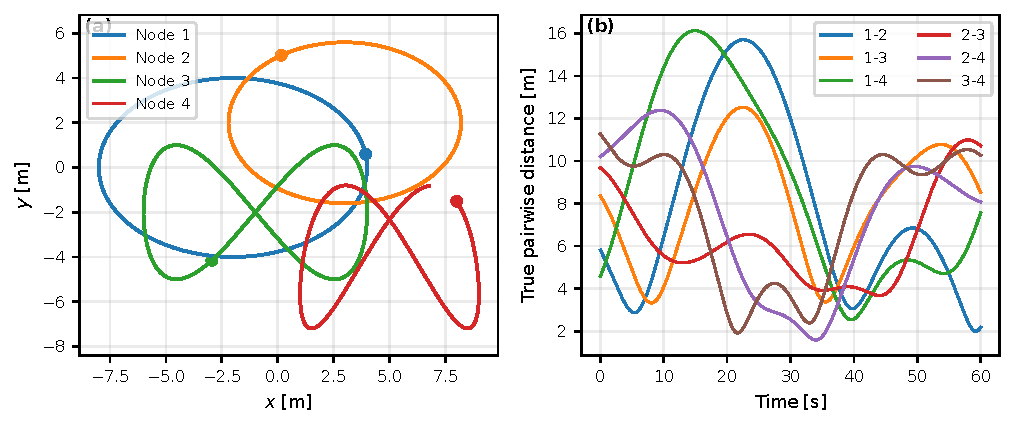
\includegraphics[width=0.98\textwidth]{figures/phase2/p2a_truth_and_geometry.pdf}
    \caption{P2A trajectory-first four-node benchmark. (a) Smooth global paths and known start locations. (b) Time-varying true distance of all six possible pairwise UWB links.}
    \label{fig:p2a_truth_geometry}
\end{figure}

The kinematics remain intentionally moderate: speed ranges from about \SI{0.185}{m/s} to \SI{0.818}{m/s}, maximum body-acceleration magnitude is approximately \SI{0.137}{m/s^2}, and the largest yaw rate is approximately \(39.6^\circ/\mathrm{s}\). Figure~\ref{fig:p2a_truth_imu} verifies the generated speed and ideal IMU signal histories directly.

\begin{figure}[htbp]
    \centering
    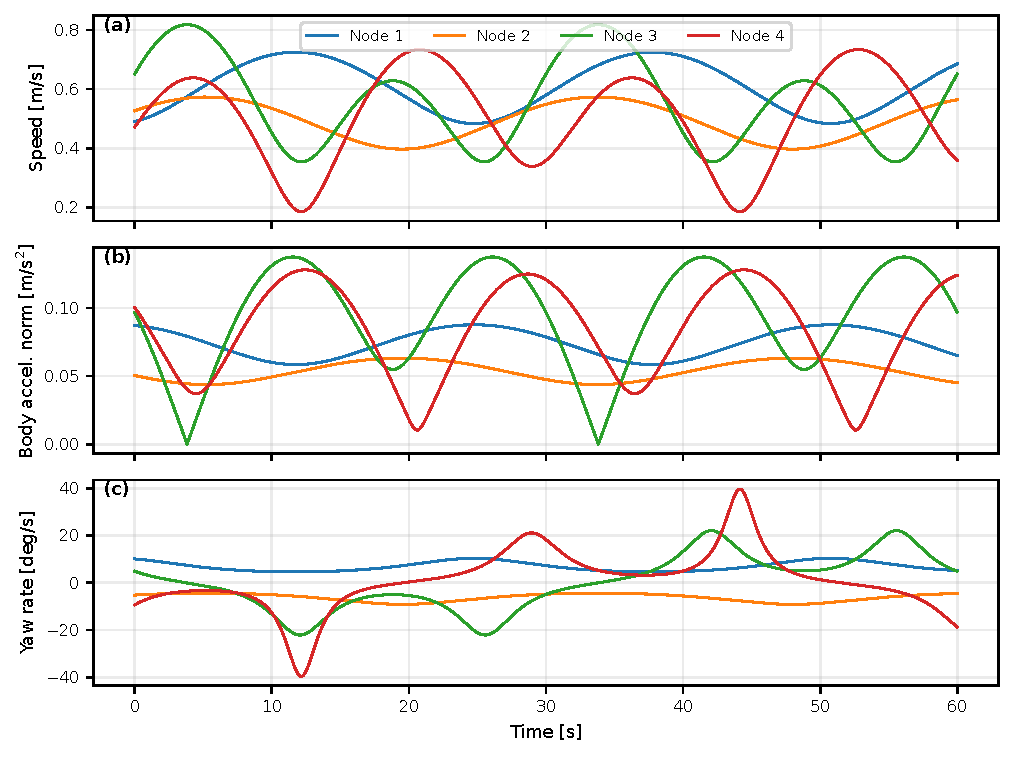
\includegraphics[width=0.98\textwidth]{figures/phase2/p2a_truth_imu_signals.pdf}
    \caption{P2A truth-derived motion signals. (a) Node speed, (b) ideal horizontal body-acceleration magnitude, and (c) ideal yaw rate. The IMU signals are consequences of the prescribed global paths rather than inputs used to create them.}
    \label{fig:p2a_truth_imu}
\end{figure}

\subsection{Joint estimator and communication references}
Each node uses
\begin{equation}
    \bm{x}_{i,k}
    =
    \begin{bmatrix}
        p_{x,i,k} & p_{y,i,k} & v_{x,i,k} & v_{y,i,k} & \psi_{i,k}
    \end{bmatrix}^{\top}.
\end{equation}
The centralized benchmark estimator stacks the four node states into a 20-state joint EKF. Position and yaw are initialized at their known truth values. To avoid silently assuming the entire kinematic state is exact, each initial velocity component receives a matched Gaussian perturbation with standard deviation \SI{0.05}{m/s}.

For a UWB exchange between nodes \(i\) and \(j\),
\begin{equation}
    z_{ij,k}
    =
    \left\|\bm{p}_{i,k}-\bm{p}_{j,k}\right\|_2+\nu_{ij,k},
    \qquad
    \sigma_{\mathrm{UWB}}=\SI{0.12}{m}.
\end{equation}
The range Jacobian contains equal and opposite position components for the two endpoints, so each measurement updates both nodes and creates cross-node covariance.

P2A compares two matched references over 20 stochastic seeds:
\begin{enumerate}
    \item \textbf{IMU only:} no UWB exchanges;
    \item \textbf{full communication:} all six links at \SI{10}{Hz}.
\end{enumerate}
The latter uses 600 UWB opportunities over \SI{60}{s}, i.e.
\begin{equation}
    C_{\mathrm{comm}}=600\binom{4}{2}=3600
\end{equation}
pairwise range exchanges and normalized communication ratio \(\rho_{\mathrm{comm}}=1\).

\subsection{Representative node behavior}
Figure~\ref{fig:p2a_rep_errors} shows one matched realization. Without ranging, independent inertial errors accumulate differently for the four nodes. Full all-pairs ranging strongly suppresses the differential position error, and the four corrected node errors become much more similar because the fleet is constrained as a coupled relative configuration.

\begin{figure}[htbp]
    \centering
    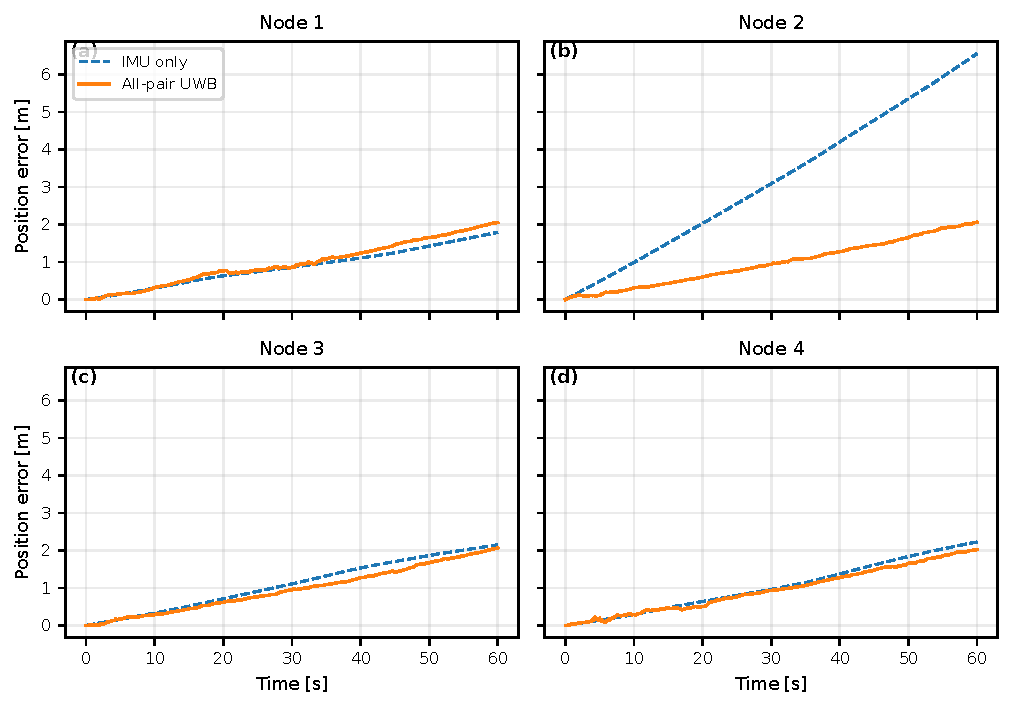
\includegraphics[width=0.98\textwidth]{figures/phase2/p2a_representative_node_errors.pdf}
    \caption{Representative P2A position-error histories for all four nodes. The same initial state and IMU realization are used for IMU-only and full-communication estimation.}
    \label{fig:p2a_rep_errors}
\end{figure}

The individual curves need not improve at every instant. For each node, its absolute position error is the sum of the fleet-centroid error and its error relative to that centroid:
\begin{equation}
    \hat{\bm p}_{i,k}-\bm p_{i,k}
    =
    \bar{\bm e}_k+\tilde{\bm e}_{i,k}.
\end{equation}
Pairwise ranges mainly reduce the second term; they provide no direct measurement of a common translation of the fleet. In the IMU-only realization, a node's relative error can partly cancel the centroid error, making its absolute error temporarily small. Correcting that relative error can remove this favorable cancellation, so the cooperative trace for that node can lie above its IMU-only trace even as the fleet geometry improves. This explains the intervals for Node~1 in Fig.~\ref{fig:p2a_rep_errors}; it does not imply that ranging is systematically harmful to Node~1.

The plot shows one matched stochastic realization, and cooperation carries no guarantee of a smaller absolute error for every node at every time. The aggregate comparison below establishes the improvement in fleet RMSE across all 20 seeds. The centroid and relative-shape decomposition then identifies which error component the UWB measurements actually reduce.

\subsection{Aggregate 20-seed localization result}
Table~\ref{tab:p2a_aggregate} gives the compact numerical result. Full all-pairs UWB improves absolute fleet position RMSE in all 20 matched seeds and reduces the mean fleet RMSE from \SI{2.322}{m} to \SI{1.058}{m}, a reduction of approximately \(54.5\%\). The mean worst-node RMSE decreases from \SI{3.238}{m} to \SI{1.071}{m}, a reduction of approximately \(66.9\%\).

\begin{table}[htbp]
    \centering
    \caption{P2A 20-seed localization result.}
    \label{tab:p2a_aggregate}
    \begin{tabular}{lrr}
        \toprule
        Metric & IMU only & All-pairs UWB, 10 Hz\\
        \midrule
        Fleet position RMSE [m] & \(2.322\pm0.605\) & \(\mathbf{1.058\pm0.451}\)\\
        Fleet RMSE p95 across seeds [m] & 3.224 & 1.641\\
        Mean worst-node RMSE [m] & 3.238 & 1.071\\
        Centroid RMSE [m] & 1.057 & 1.056\\
        Relative-shape RMSE [m] & 2.027 & 0.046\\
        UWB exchanges per run & 0 & 3600\\
        \bottomrule
    \end{tabular}
\end{table}

Figure~\ref{fig:p2a_aggregate_perf} provides the more detailed time-domain and paired-seed view. The all-pairs reference has lower fleet RMSE than IMU-only propagation in every matched run.

\begin{figure}[htbp]
    \centering
    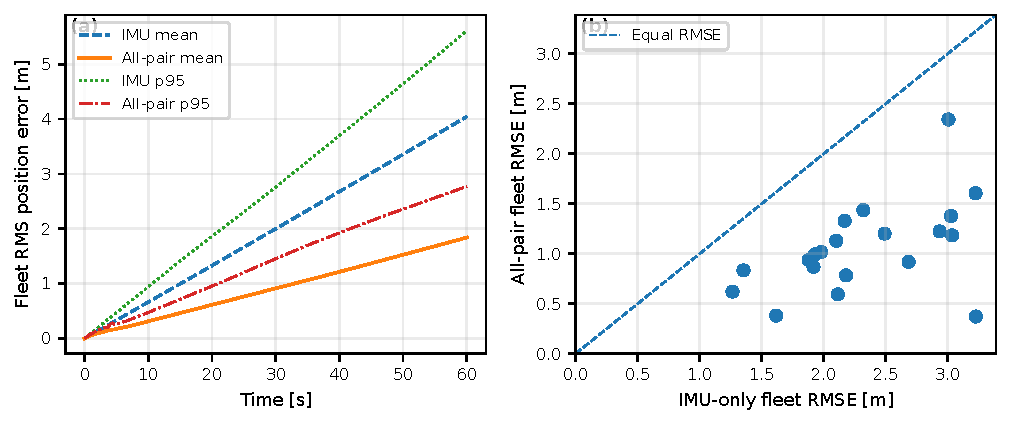
\includegraphics[width=0.98\textwidth]{figures/phase2/p2a_aggregate_performance.pdf}
    \caption{Aggregate P2A performance. (a) Mean and 95th-percentile fleet RMS position-error histories across 20 seeds. (b) Paired seed-level fleet RMSE; points below the equality line favor full communication.}
    \label{fig:p2a_aggregate_perf}
\end{figure}

UWB does not materially improve yaw in this benchmark: the mean fleet yaw RMSE is about \(0.047^\circ\) for IMU-only propagation and \(0.057^\circ\) for full communication. This is expected because the scalar pairwise ranges directly constrain position, while yaw is influenced only indirectly through state cross-covariances and motion.

\subsection{What pairwise UWB can and cannot correct}
The most important P2A result is exposed by decomposing position error into common translation and relative fleet shape. Define the fleet-centroid error
\begin{equation}
    \bar{\bm e}_k
    =
    \frac{1}{N}
    \sum_{i=1}^{N}
    \left(\hat{\bm p}_{i,k}-\bm p_{i,k}\right),
\end{equation}
and centered relative errors
\begin{equation}
    \tilde{\bm e}_{i,k}
    =
    \left(\hat{\bm p}_{i,k}-\bar{\hat{\bm p}}_k\right)
    -
    \left(\bm p_{i,k}-\bar{\bm p}_k\right).
\end{equation}
Pairwise ranges are invariant to a common translation of the entire fleet. Consequently, they can strongly constrain the relative configuration but cannot directly remove common-mode global drift.

The experiment shows exactly this behavior. Mean centroid RMSE is essentially unchanged:
\begin{equation}
    \SI{1.0566}{m}
    \;\rightarrow\;
    \SI{1.0564}{m},
\end{equation}
whereas relative-shape RMSE collapses from
\begin{equation}
    \SI{2.027}{m}
    \;\rightarrow\;
    \SI{0.0456}{m},
\end{equation}
a reduction of approximately \(97.8\%\). Figure~\ref{fig:p2a_decomp} shows the same distinction over time.

\begin{figure}[htbp]
    \centering
    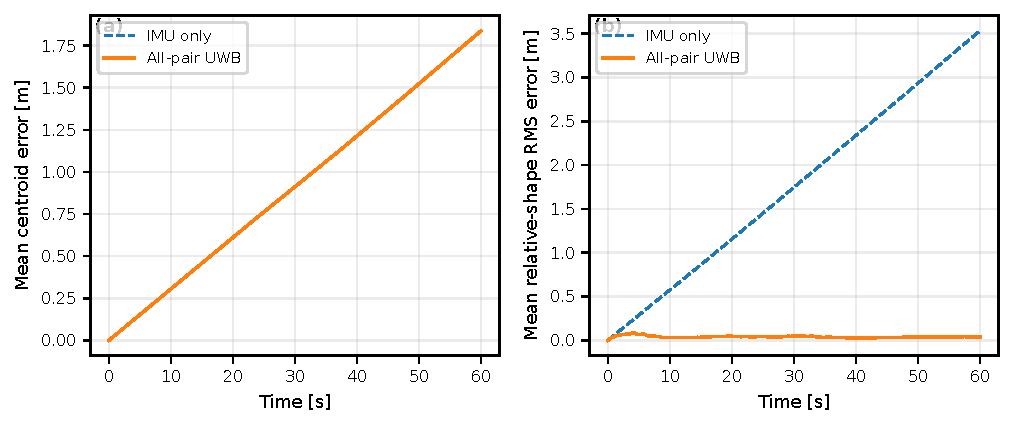
\includegraphics[width=0.98\textwidth]{figures/phase2/p2a_error_decomposition.pdf}
    \caption{P2A infrastructure-free error decomposition. (a) Mean fleet-centroid/common-translation error. (b) Mean centered relative-shape error. Full pairwise UWB nearly eliminates differential fleet deformation but leaves the common global translation mode essentially unchanged.}
    \label{fig:p2a_decomp}
\end{figure}

This is not a weakness of the EKF implementation; it is a structural property of an infrastructure-free pairwise-ranging network. Known initial poses establish the initial global frame, but subsequent pairwise ranges contain no direct information about a uniform translation of every node. The absolute fleet RMSE therefore approaches a common-mode floor even under maximum communication.

\subsection{Covariance diagnostic}
Figure~\ref{fig:p2a_consistency} compares the representative full-communication position error with the EKF position-covariance scale for each node. This is retained as an estimator diagnostic rather than as a formal statistical consistency proof. The main purpose is to make covariance behavior visible before that covariance is later used for information-aware link scheduling.

\begin{figure}[htbp]
    \centering
    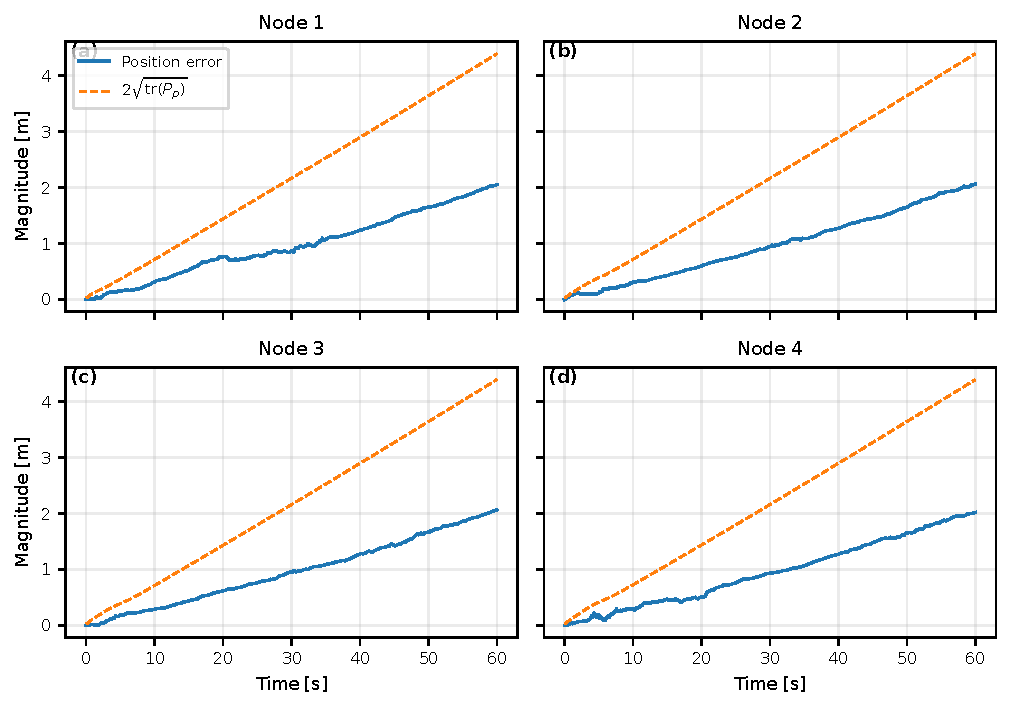
\includegraphics[width=0.98\textwidth]{figures/phase2/p2a_ekf_consistency.pdf}
    \caption{Representative P2A EKF covariance diagnostic. Per-node position error is shown together with twice the radial covariance scale \(2\sqrt{\operatorname{tr}(P_p)}\).}
    \label{fig:p2a_consistency}
\end{figure}

\subsection{P2A decision and handoff}
P2A establishes a suitable canonical benchmark:
\begin{itemize}
    \item the trajectory-first sensor generation is numerically self-consistent;
    \item the four-node geometry is smooth, visually interpretable, and time varying;
    \item full all-pairs UWB materially improves absolute fleet RMSE in every seed;
    \item pairwise UWB almost completely suppresses relative fleet deformation;
    \item a common global-translation error remains because the network has no absolute ranging reference.
\end{itemize}

The next step is therefore \textbf{P2B: uniform communication-rate reduction}. The same trajectories, seeds, estimator, and all-pairs topology should be retained while the UWB rate is reduced from the \SI{10}{Hz} reference. The primary output will be the first empirical fleet-error versus normalized-communication frontier. The centroid/relative-shape decomposition should remain first-class because communication can only trade against error modes that pairwise UWB can observe.
